\section{Solution strategy}
When solving a complex problem as this problem of developing a vision system for a robot, it is possible to dedicate time and resources to a solution approach that turns out not to achieve the desired result. It is therefore important to come up with a solution strategy which ensures the available time and resources are not wasted. The purpose of this section is to present the solution strategy for this report.
%Vision control of robots has become quite effective and is widely used in modern production, especially in packaging operations. This is due to the increase in usability, since it used be complicated to setup the communication between the vision and the robot. The purpose of this section is firstly to investigate if a standard commercial visual solution is able to assemble the assembly. Secondly it will present the strategy for solving how to control the Cobra with a vision system and assemble the assembly.


% \subsection{ABB Delta Robot}
% ABB has developed a standard solution for pick and place using the delta robot design, shown on figure \ref{fig_abb_delta}. One specific compeny using this solution is Honeytop Speciality Foods Ltd, who uses the delta robot with a suction tool, as end effector, to pick up and stack honey pancakes, as shown on figure \ref{fig_abb_pancakes}. \citep{pancakes}
%
% \begin{figure}[htbp!]
% \centering
% \begin{subfigure}[t]{0.46\textwidth}
% \centering
%   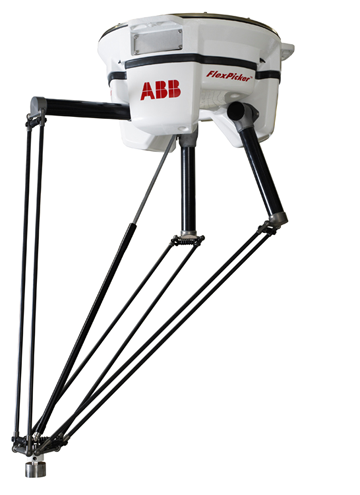
\includegraphics[width=0.45\textwidth,]{prob_ana_delta}
%   \caption{The ABB delta Robot \citep{pancakes_pic}}
%   \label{fig_abb_delta}
%   \end{subfigure}~~
% \begin{subfigure}[t]{0.46\textwidth}
% \centering
% %  \captionsetup{width=\textwidth}
%   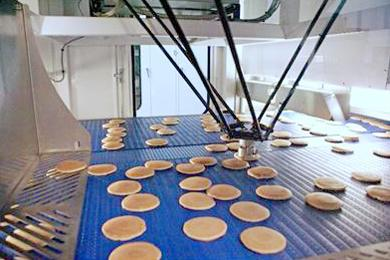
\includegraphics[width=\textwidth]{prob_ana_pancakes}
%   \caption{The Delta robot performing the pick and place operation of the pancakes \citep{pancakes}}
%   \label{fig_abb_pancakes}
%   \end{subfigure}
%   \caption{ABB's solution for a pick and place operation}
% \end{figure}
% \noindent The specific delta robot shown on the pictures is able to achieve large accelerations but the maximum payload is limited to a few kilos. The setup for the production line is a shown on figure \ref{fig_sketch_production}.
% \begin{figure}[htbp!]
% \centering
%   \begin{tikzpicture}
%   \coordinate (box_top) at (1,0);
%
%   \coordinate (box_bottom) at (3,4);
%   \coordinate (conveyor_top) at (-1,1);
%   \coordinate (conveyor_bottom) at (10,3);
%   \coordinate (place_top) at (4.5,3.2);
%   \coordinate (place_bottom) at (10,4.2);
%   \draw [dashed] (conveyor_top) rectangle (conveyor_bottom);
%   \draw[fill=yellow] (1,1.5) circle (1em);
%    \draw[fill=yellow] (3,2.5) circle (1em);
%   \draw[fill=white] (box_top) rectangle (box_bottom);
%     \draw (place_top) rectangle (place_bottom);
%   \draw (box_top)+(1,2) node{Camera} ;
%   \draw[fill=yellow] (-0.5,1.5) circle (1em);
%   \draw[fill=yellow] (.5,2.5) circle (1em);
%    \draw[fill=yellow] (3.5,1.5) circle (1em);
%     \draw[fill=yellow] (4.5,2.5) circle (1em);
%      \draw[fill=yellow] (5,3.7) circle (1em);
%      \draw[fill=yellow] (6,3.7) circle (1em);
%   \draw[fill=yellow] (7,3) circle (1em);
%   \draw[fill=gray] (7,3) circle (0.7em);
%   \draw (conveyor_top)+(6,-0.5) node{Conveyor belt};
%   \draw (place_top)+(3,1.2) node{Drop-off belt};
%
%   \end{tikzpicture}
%   \caption{Sketch of the production line, where the yellow circles are the pancakes and the gray circle indicates the suction tool grabbing the pancakes}
%   \label{fig_sketch_production}
% \end{figure}\newline
% The pancakes passes under a the camera, which is shielded from the light disturbances, such that the pancakes are only exposed to the light inside the shield. The light inside the shield is adjusted to give the picture the camera sees maximum contrast, and thereby the vision system is able to detect position and orientation of the pancakes. From this information, and with knowledge about the speed of the conveyor belt, the vision system is able to preciously predict, where a specific pancake will be on the conveyor belt at a given time. This prediction is forwarded to the robot, such that the robot can pick up the specific pancake and place it at the drop-off belt.\newline
% In an article by ABB, there is some guidelines for how to optimise a production like the above, the key points in this article for the vision detection are: \citep{abb_delta}
% \begin{itemize}
%   \item Adjusting the lighting inside the shield for the specific object, such that maximum contrast is achieved. This ensures the vision system is able to detect the predefined object
%   \item The conveyor belt color should be different than the object's color, preferably a contrast color
%   \item In some production lines, preconditioning will improve the vision performance, in the case of the pancakes, this is ensuring there is not to much overlap of the pancakes, such that the vision system is not able to detect the bottom pancake.
% \end{itemize}
% From these requirements, it is concluded that the ABB solution is not flexible enough to fulfil the desires of Aaborg University. It is therefore necessary to develop a modification for the test setup and the necessary software. 

\subsection{Lean startup method}\label{sub_lean_startup}
To summarise; The test system consist of a robot and conveyor belt and the idea is all parts of the assembly is located on the conveyor and the conveyor belt's velocity is allowed to change. The goal is a visual system should identify position, orientation and speed of the parts and forward this information to a planner tool to ensure the assembly is correctly assembled. Finally it is necessary to derive a control strategy, which ensures the robot tracks the planned trajectory and performs the pick-up operation. Solving this task as described is complicated and leads to complications. To avoid this, one approach is to use the methodology called the lean startup method, and the idea is to follow the loop shown on figure \ref{fig_lean_startup}
\begin{figure}[htbp!]
\centering
\begin{tikzpicture}[>=stealth',shorten >=1pt,auto]
\tikzstyle{circ} = [draw, fill=blue!40, circle, node distance = 2cm,minimum size=4em]
\tikzstyle{input} = [coordinate]
%\tikzstyle{pinstyle} = [pin edge={to-,thin,black}]
\node[circ] (build) {Build};
\node[circ,left of=build,node distance = 4cm](learn) {Learn};
\node[input,left of=build,node distance = 2cm](guide) {};
\node[circ,below of = guide,node distance = 4cm](meas){Measure};

\draw[->] (build) edge[bend left = 40] (meas);
\draw[->] (meas) edge[bend left = 40] (learn);
\draw[->] (learn) edge[bend left = 40] (build);
\end{tikzpicture}
  \caption{Lean startup ideology}
\label{fig_lean_startup}
\end{figure}\newline
With the context of this report, the approach is to spilt the problem into modules and then define a simple task for the modules, solve it and learn from the procedure. At each iteration the complexity of the modules' tasks are increase until the original goal is solved. The modules for this report are:
\begin{enumerate}
  \item The modifications for the test setup; type of and number of cameras and lighting inside the cage \label{item_test}
  \item Assembling of the assembly; number of parts used and color of the parts  \label{item_assem}
  \item Conveyor belt; the maximum velocity of the conveyor belt and what kind of changes can happen to the velocity \label{item_conve}
  \item Visual system; detecting the parts on the conveyor belt and deriving position, orientation and velocity \label{item_vis}
  \item Control strategy and trajectory tracking for the robot; with the information from the visual system, it is necessary to plan a trajectory for the robot and control strategy to ensure the robot is tracking the trajectory \label{item_control}
  \item Communication between visual system and the robot control unit; how the control strategy output is translated into signals for the robot, while still ensuring the system bandwidth is sufficient \label{item_com}
   
\end{enumerate}
Module \ref{item_test} to \ref{item_conve} are physical modules, where module \ref{item_conve} is defined to challenge the solution for each iteration. The modules \ref{item_vis} to \ref{item_com} are software modules and should only depend on some specific inputs and give specific outputs such that it is possible to change them if the need arises. 



























 
